%
% ---------------------------------------------------
%
% Trabajo Fin de Grado:
% Author: Laura Padrón Jorge <gonzalezsuarezivan@gmail.com>
% Author: F. de Sande fsande@ull.es
% Fichero: main.tex
%
% ----------------------------------------------------
%
\documentclass[spanish,a4paper,12pt,oneside]{extreport}
%\documentclass[a4paper, twoside, 12pt]{book}
\usepackage[a4paper]{geometry}
\usepackage[spanish]{babel}
\usepackage[utf8]{inputenc}
%\usepackage{lscape}
\usepackage{pdflscape}
%%%%%%%%%%%%%%%%%%%%%%%%%%%%%%%%%%%%%%%%%%%%%%%%%%%%%%%%%%%%%%%%%%%%%%%%%%%%%%%%%%%%%%%%%%%%
% Next 3+3 lines select PDF or PS output (comment as apropriate)
% To switch from PDF and PS comment/uncomment here and change Makefile
\usepackage[pdftex]{color}
\usepackage[pdftex]{graphicx}
\graphicspath{{images/}}
%\usepackage[dvips]{color}
%\usepackage[dvips]{graphicx}
\usepackage{epsfig}
%\graphicspath{{images/eps/}}
%Añadidos BulletPoint
\usepackage{floatrow}
%%%%%%%%%%%%%%%%%%%%%%%%%%%%%%%%%%%%%%%%%%%%%%%%%%%%%%%%%%%%%%%%%%%%%%%%%%%%%%%%%%%%%%%%%%%%
\usepackage{algorithmic}
\usepackage[pdftex=true,colorlinks=false,urlcolor=blue,plainpages=false,pagebackref=true,citecolor=red]{hyperref} %hiperenlaces y backcites 
%%%%%%%%%%%%%%%%%%%%%%%%%%%%%%%%%%%%%%%%%%%%%%%%%%%%%%%%%%%%%%%%%%%%%%%%%%%%%%%%%%%%%%%%%%%%
% Comandos para escribir "siempre igual"
\newcommand{\MIMIC}{\texttt{Panel de estado del instrumento científico MIRADAS.}}



%%% Traducimos el pseudocodigo
\renewcommand{\algorithmicwhile}{\textbf{mientras}}
\renewcommand{\algorithmicend}{\textbf{fin}}
\renewcommand{\algorithmicdo}{\textbf{hacer}}
\renewcommand{\algorithmicif}{\textbf{si}}
\renewcommand{\algorithmicthen}{\textbf{entonces}}
\renewcommand{\algorithmicrepeat}{\textbf{repetir}}
\renewcommand{\algorithmicuntil}{\textbf{hasta que}}
\renewcommand{\algorithmicelse}{\textbf{en otro caso}}
\renewcommand{\algorithmicfor}{\textbf{para}}

%%%%%%%%%%%%%%%%% Creamos un entorno para listar código fuente %%%%%%%%%%%%%%%
\newenvironment{sourcecode}
{\begin{list}{}{\setlength{\leftmargin}{1em}}\item\scriptsize\bfseries}
{\end{list}}

\newenvironment{littlesourcecode}
{\begin{list}{}{\setlength{\leftmargin}{1em}}\item\tiny\bfseries}
{\end{list}}

\newenvironment{summary}
{\par\noindent\begin{center}\textbf{Abstract}\end{center}\begin{itshape}\par\noindent}
{\end{itshape}}

\newenvironment{keywords}
{\begin{list}{}{\setlength{\leftmargin}{1em}}\item[\hskip\labelsep \bfseries Keywords:]}
{\end{list}}

\newenvironment{palabrasClave}
{\begin{list}{}{\setlength{\leftmargin}{1em}}\item[\hskip\labelsep \bfseries Palabras clave:]}
{\end{list}}


%%%%%%%%%%%%%%%%%%%%%%%%%%%%%%%%%%%%%%%%%%%%%%%%%%%%%%%%%%%%%%%%%%%%%%%%%%%%%%%
\definecolor{marron}       {rgb}{0.496, 0.203, 0.152}
\definecolor{verde-claro}  {rgb}{0.625, 0.734, 0.199}
\definecolor{oscuro}       {rgb}{0.187, 0.141, 0.285}
\definecolor{gris}     	   {rgb}{0.500, 0.500, 0.500}
\definecolor{bgd-listings} {rgb}{0.999, 0.999, 0.900}
\definecolor{gray97}{gray}{.97}
\definecolor{gray75}{gray}{.75}
\definecolor{gray45}{gray}{.45}
\definecolor{gray}{gray}{.45}
%%%%%%%%%%%%%%%%%%%%%%%%%%%%%%%%%%%%%%%%%%%%%%%%%%%%%%%%%%%%%%%%%%%%%%%%%%%%%%%%%%%%%%%%%%%%
%%% Code Listings
%\usepackage{listings} 
%\lstloadlanguages{python,C}
\definecolor{Brown}{cmyk}{0,0.81,1,0.60}
\definecolor{OliveGreen}{cmyk}{0.64,0,0.95,0.40}
\definecolor{CadetBlue}{cmyk}{0.62,0.57,0.23,0}
\definecolor{lightlightgray}{gray}{0.9}
%%%%%%%%%%%%%%%%%%%%%%%%%%%%%%%%%%%%%%%%%%%%%%%%%%%%%%%%%%%%%%%%%%%%%%%%%%%%%%%%%%%%%%%%%%%
%Evitar partir palabras al final de la línea
\hyphenpenalty=10000
\tolerance=1000
%%%%%%%%%%%%%%%%%%%%%%%%%%%%%%%%%%%%%%%%%%%%%%%%%%%%%%%%%%%%%%%%%%%%%%%%%%%%%%%%%%%%%%%%%%%%
% Para listados de código
\usepackage{listings}
\lstloadlanguages{C}

% Definiendo colores para los listados de código fuente - Univ. Deusto
\definecolor{violet}{rgb}{0.5,0,0.5}
\definecolor{navy}{rgb}{0,0,0.5}
\definecolor{hellgelb}{rgb}{1,1,0.8}
\definecolor{colKeys}{rgb}{0,0,1}
\definecolor{colIdentifier}{rgb}{0,0,0}
\definecolor{colComments}{rgb}{1,0,0}
\definecolor{colString}{rgb}{0,0.5,0}

%\lstset{morekeywords={pragma copy\_in copy\_out copy omp parallel private reduction shared hicuda loop\_partition over\_tblock over\_thread}}
\lstset{
        float=tbhp,
		    language = Java,
				morekeywords={llc,reduction_type,nc_result,
				              hicuda,global,alloc,shape,kernel,thread,loop_partition,tblock,over_tblock,over_thread,kernel_end,copyout,free,
											data,region,
											task,input,inout,output,
				              pragma,omp,parallel,reduction,private,shared,target,device,copy_in,copy_out,
				              acc,kernels,loop,copyin,copy,pcopy,pcopyin,collapse,gang,worker,independent},
				%\emph      ={omp,parallel,reduction,private,shared},
				emphstyle=\textbf,
        %basicstyle=\ttfamily\tiny,
        basicstyle=\ttfamily\scriptsize,
        identifierstyle=\color{colIdentifier},
        keywordstyle=\color{colKeys},
        stringstyle=\color{colString},
        commentstyle=\color[rgb]{0.133,0.545,0.133},
        columns=flexible,
        tabsize=4,
        frame=single,
        extendedchars=true,
        showspaces=false,
        showstringspaces=false,
        numbers=left,
        numberstyle=\tiny,
        breaklines=true,
        backgroundcolor=\color{lightlightgray},
        breakautoindent=true,
        captionpos=b
}

%\renewcommand{\lstlistingname}{Listing} % Los títulos de los códigos insertados se denotan con Ejemplo...   

% Otro formato más bonito para código fuente
\newcommand{\codigofuente}[3]{%
  \lstlisting[language=#1,caption={#2}]{#3}%
}
%%%%%%%%%%%%%%%%%%%%%%%%%%%%%%%%%%%%%%%%%%%%%%%%%%%%%%%%%%%%%%%%%%%%%%%%%%%%%%%
\begin{document}
\renewcommand{\lstlistingname}{Listado}% Listing -> Listado de código
%%%%%%%%%%%%%%%%%%%%%%%%%%%%%%%%%%%%%%%%%%%%%%%%%%%%%%%%%%%%%%%%%%%%%%%%%%%%%%%
% First Page
%%%%%%%%%%%%%%%%%%%%%%%%%%%%%%%%%%%%%%%%%%%%%%%%%%%%%%%%%%%%%%%%%%%%%%%%%%%%%%%

\pagestyle{empty}
\thispagestyle{empty}


\newcommand{\HRule}{\rule{\linewidth}{1mm}}
\setlength{\parindent}{0mm}
\setlength{\parskip}{0mm}

\vspace*{\stretch{0.5}}

\begin{center}

\includegraphics[scale=0.8]{images/logo_vertical}\\[10mm]
{\Huge Trabajo de Fin de Grado}
\end{center}

\HRule
\begin{flushright}
        {\Huge \MIMIC{}} \\[2.5mm]
        {\Large Javier Alberto Martín} \\[5mm]


\end{flushright}
\HRule
\vspace*{\stretch{2}}
\begin{center}
  \Large La Laguna, \today
\end{center}

\setlength{\parindent}{5mm}

%%%%%%%%%%%%%%%%%%%%%%%%%%%%%%%%%%%%%%%%%%%%%%%%%%%%%%%%%%%%%%%%%%%%%%%%%%%%%%%
% Signature page (add the official stamp)
%%%%%%%%%%%%%%%%%%%%%%%%%%%%%%%%%%%%%%%%%%%%%%%%%%%%%%%%%%%%%%%%%%%%%%%%%%%%%%%
\newpage
%\cleardoublepage
\thispagestyle{empty}

D. {\bf Francisco de Sande González}, con DNI nº 42.067.050-G
profesor Titular de Universidad adscrito al Departamento de Ingeniería Informática y de Sistemas
de la Universidad de La Laguna, como tutor

\bigskip

\bigskip
\bigskip
{\bf C E R T I F I C A}

\bigskip
\bigskip
\bigskip
Que la presente memoria titulada:

\bigskip
``{\it \MIMIC{}}''

\bigskip
\bigskip
\bigskip
%Cambiar
\noindent ha sido realizada bajo su dirección por D. {\bf Javier Alberto Martín},
con DNI nº 45.733.473-C

\bigskip
\bigskip

Y para que así conste, en cumplimiento de la legislación vigente y a los efectos
oportunos firman la presente en La Laguna a \today

%\cleardoublepage
\newpage
%%%%%%%%%%%%%%%%%%%%%%%%%%%%%%%%%%%%%%%%%%%%%%%%%%%%%%%%%%%%%%%%%%%%%%%%%%%%%%%
\thispagestyle{empty}

{ \flushright

\begin{LARGE}
Agradecimientos
\end{LARGE}

\hspace{3mm}

\begin{large}


\hspace{3mm}


Mis agradecimientos bla bla bla XXX



\end{large}

}

%%%%%%%%%%%%%%%%%%%%%%%%%%%%%%%%%%%%%%%%%%%%%%%%%%%%%%%%%%%%%%%%%%%%%%%%%%%%%%%%%
\newpage

\begin{huge}
Licencia
\end{huge}

\bigskip
%* Si quiere permitir que se compartan las adaptaciones de tu obra mientras se comparta de la misma manera
%y NO quieres permitir usos comerciales de tu obra indica:

\begin{center}

\includegraphics[scale=1.5]{images/by-nc-sa_88x31}\\[10mm]
{\Large \copyright~Esta obra está bajo una licencia de Creative Commons Reconocimiento-NoComercial-CompartirIgual 4.0 Internacional.
}
\end{center}


%%%%%%%%%%%%%%%%%%%%%%%%%%%%%%%%%%%%%%%%%%%%%%%%%%%%%%%%%%%%%%%%%%%%%%%%%%%%%%%
\newpage  %\cleardoublepage
\begin{abstract}
{\em

Este documento constituye el trabajo de investigación del alumno durante el proceso de desarrollo de un panel de estados para el instrumento MIRADAS mediante el uso de una de las tecnologías más recientes y menos conocidas en el mercado actual: los Beacons.

\bigskip
Partimos de los conocimientos de programación en \textit{Java} adquiridos en la asignatura: \textit{``Diseño arquitectónico y patrones''} cursada en el 
itinerario de Ingeniería del Software. Esta asignatura, impartida en el tercer curso del Grado en Ingeniería Informática de la Universidad de La Laguna, ha sido la que ha sentado los fundamentos a partir de los cuáles se ha desarrollado la aplicación.

\bigskip
Durante este proyecto, el alumno ha conseguido adquirir independencia en su trabajo, visión y planificación realizando tareas de investigación, desarrollo y documentación, que han dado como resultado la obtención de conocimientos durante el proceso de trabajo.

\bigskip 
También se ha investigado la reciente tecnología ``beacon'' que si bien aún no tiene un impacto muy grande, en un futuro inmediato se espera que se empiece a utilizar con naturalidad en distintos ámbitos: turismo, comercio, enseñanza, etc.

}
\begin{palabrasClave}
Java, GTC, MIRADAS... XXX (ir metiendo)
\end{palabrasClave}

\end{abstract}
%%%%%%%%%%%%%%%%%%%%%%%%%%%%%%%%%%%%%%%%%%%%%%%%%%%%%%%%%%%%%%%%%%%%%%%%%%%%%%%

%%%%%%%%%%%%%%%%%%%%%%%%%%%%%%%%%%%%%%%%%%%%%%%%%%%%%%%%%%%%%%%%%%%%%%%%%%%%%%%
\newpage  %\cleardoublepage
\begin{summary}
{\em

The aim of the project has been the development of an application for Android devices that uses beacon technology for some of its main features.

\bigskip
Based on the knowledge of \textit{Java} programming obtained in the subject: \textit{``Architectural Design and Patterns''} studied in the
Software Engineering Branch (given in third year of Computing Engineering degree from \textit{``La Universidad de La Laguna''}). In this work we have acquired the basic knowledge needed to develop Android applications introducing us in the development of applications related to beacon technology.

\bigskip
Moreover, the student has learned independence in her work and gained vision and scheduling aptitudes, developing different labors of research, development and documentation that have come to give her a wide knowledge during the development of this project.

\bigskip
Apart from all this, it's of great value for the student to get to know this new beacon technology. I have investigated and learned from this new technology, which at the moment is not well known, but in the close future it is expected to get more attention in different sectors, such as tourism, trading or learning.
}

\begin{keywords}
Application for Android, Java, mobile devices, programming, Beacons.
\end{keywords}

\end{summary}
%%%%%%%%%%%%%%%%%%%%%%%%%%%%%%%%%%%%%%%%%%%%%%%%%%%%%%%%%%%%%%%%%%%%%%%%%%%%%%%

%%%%%%%%%%%%%%%%%%%%%%%%%%%%%%%%%%%%%%%%%%%%%%%%%%%%%%%%%%%%%%%%%%%%%%%%%%%%%%%
\newpage{\pagestyle{empty}}
\thispagestyle{empty}

%%%%%%%%%%%%%%%%%%%%%%%%%%%%%%%%%%%%%%%%%%%%%%%%%%%%%%%%%%%%%%%%%%%%%%%%%%%%%%%


\pagestyle{myheadings} %my head defined by markboth or markright
% No funciona bien \markboth sin "twoside" en \documentclass, pero al
% ponerlo se dan un montón de errores de underfull \vbox, con lo que no se
% ha puesto.
\markboth{Javier Alberto Martín}{BulletPoint}

%%%%%%%%%%%%%%%%%%%%%%%%%%%%%%%%%%%%%%%%%%%%%%%%%%%%%%%%%%%%%%%%%%%%%%%%%%%%%%%
%Numeracion en romanos
\renewcommand{\thepage}{\roman{page}}
\setcounter{page}{1}

%%%%%%%%%%%%%%%%%%%%%%%%%%%%%%%%%%%%%%%%%%%%%%%%%%%%%%%%%%%%%%%%%%%%%%%%%%%%%%%

\tableofcontents

%%%%%%%%%%%%%%%%%%%%%%%%%%%%%%%%%%%%%%%%%%%%%%%%%%%%%%%%%%%%%%%%%%%%%%%%%%%%%%%
\newpage{\pagestyle{empty}}

\listoffigures

%%%%%%%%%%%%%%%%%%%%%%%%%%%%%%%%%%%%%%%%%%%%%%%%%%%%%%%%%%%%%%%%%%%%%%%%%%%%%%%
\newpage{\pagestyle{empty}}

%\listoftables

%%%%%%%%%%%%%%%%%%%%%%%%%%%%%%%%%%%%%%%%%%%%%%%%%%%%%%%%%%%%%%%%%%%%%%%%%%%%%%%
\newpage{\pagestyle{empty}}

%%%%%%%%%%%%%%%%%%%%%%%%%%%%%%%%%%%%%%%%%%%%%%%%%%%%%%%%%%%%%%%%%%%%%%%%%%%%%%%
%Numeracion a partir del capitulo I
\renewcommand{\thepage}{\arabic{page}}
\setcounter{page}{1}


% ==========================================================
% --------               Capítulos                ----------
% --------    Estan en el directorio capitulos/   ----------
% ==========================================================
% ---------------------------------------------------
%
% Proyecto de Final de Carrera: 
% Author: Javier Alberto Martín <alu0100836400@ull.edu.es>
% Introducción
% Fichero: Prologo.tex
%
% ----------------------------------------------------

\chapter*{Prólogo}
\addcontentsline{toc}{chapter}{Prólogo} 

Este documento comprende el trabajo de investigación y desarrollo realizado por el alumno en la consecución de su Trabajo de Fin de Grado (TFG), con el que culminará sus estudios del Grado en Ingeniería Informática cursados en la Escuela Superior de Ingeniería y Tecnología (ESIT) de la Universidad de la Laguna (ULL).

El trabajo propuesto se enmarca dentro de la etapa final del desarrollo del sistema de control software destinado al instrumento científico MIRADAS, el cual se instalará en el Gran Telescopio Canarias (GTC), situado en el observatorio del Roque de Los Muchachos (ORM) en isla de La Palma. Este telescopio posee un espejo primario formado por 36 segmentos hexagonales que actúan conjuntamente como un solo espejo de un diámetro de 10.4 m. El espesor de cada segmento no excede de 8 cm.

Los instrumentos son dispositivos que se acoplan al telescopio para realizar una tarea específica con la luz reflejada por el telescopio. En el caso del instrumento MIRADAS se trata de un espectrógrafo que analiza la luz en el infrarrojo cercano donde el oscurecimiento por el gas y el polvo entre las estrellas no es un gran problema. Es un instrumento multi-objeto con una resolución espectral R = 20.000 en el rango de 1-2.5 $\mu$m. Su capacidad de multiplexación para observar varios objetos al mismo tiempo y la alta resolución espectral que se puede alcanzar determinan el atractivo de este instrumento.

El panel de estado de un instrumento representa cómo el haz de luz se ve afectado por la configuración actual del instrumento (elementos opto-mecánicos) hasta llegar al detector, así como el estado actual de la observación, si la hubiera. Esto permite a los astrónomos y operarios del telescopio visualizar la siguiente información: la trayectoria del haz de luz a través de los distintos elementos opto-mecánicos hasta llegar a su detector, el estado actual de los elementos opto-mecánicos y el progreso de la observación actual.

El software de control de MIRADAS sigue los estándares software y hardware definidos por el telescopio para permitir su integración en el sistema de control de GTC (GCS). GCS es un entorno distribuido orientado a objetos en C++, Python y Java, que ejecuta los múltiples componentes y servicios de los que está compuesto en diferentes máquinas, y utiliza el middleware CORBA para comunicarse entre ellos.

% ---------------------------------------------------
%
% Proyecto de Final de Carrera: 
% Author: Javier Alberto Martín <alu0100836400@ull.edu.es>
% Capítulo: Introducción 
% Fichero: Cap1_Introduction.tex
%
% ----------------------------------------------------


\chapter{Introducción} \label{chap:Introducción}  

\section{Objetivos}

Este TFG tiene los siguientes objetivos principales:

	
\begin{itemize}
\item  	Por un lado se pretende ampliar los conocimientos en tecnologías móviles en el sistema operativo \textit{Android} \cite{URL::Android} y en el desarrollo de aplicaciones para este sistema operativo.
\item Otro objetivo presente en este TFG es que el alumno investigue y profundice en una tecnología reciente, los \textit{beacons} \cite{URL::Beacon}.
\item Por otro lado, también se pretende que el alumno se familiarice con el uso de herramientas de control de versiones utilizando \textit{Github} \cite{URL::Github} y de edición de textos técnicos utilizando \textit{LaTeX}  \cite{URL::LaTeX}.
\item  Por último, tras las labores de investigación y recopilación de información correspondientes, se espera que el alumno aplique los conocimientos adquiridos para desarrollar una aplicación funcional que cubra las necesidades propuestas.
\end{itemize}

\section{Planificación}

\section{Conceptos previos}
% ---------------------------------------------------
%
% Trabajo de Fin de Grado. 
% Author: Laura Padrón Jorge. 
% Capítulo: Tecnologías utilizadas en el Trabajo de Fin de Grado. 
% Fichero: Cap2_Technology.tex
%
% ----------------------------------------------------
%

\cleardoublepage
\chapter{Herramientas y Tecnologías} \label{chap:Tecnologias} 

Este capítulo tiene como objetivo presentar las distintas herramientas software y tecnologías empleadas por la alumna en el desarrollo de \BulletPoint{}.

\section{Herramientas de Desarrollo}

A continuación se explicarán brevemente las distintas herramientas software utilizadas en el proyecto. 

\subsection{Android Studio}


\begin{itemize}
\item Un sistema de compilación basado en Gradle\cite{URL::Gradle} que ha simplificado tanto la inserción de dependencias de las distintas librerías que se han tenido que utilizar, como la compilación de la aplicación.
\item Un emulador rápido y fácil de utilizar que ha ayudado a visualizar las distintas pantallas durante el desarrollo aunque no ha sido de mucha utilidad para probar el funcionamiento al ser dependiente la app de la tecnología Bluetooth.
\item La facilidad para publicar cambios a aplicaciones ya funcionando sin tener que eliminar y volver a crear un nuevo APK parando la app.
\item Un sistema de visualización de las diferentes pantallas muy completo, con soporte visual para añadir componentes y cambiar atributos fácilmente.
\item Un sistema de depuración, con una interfaz sencilla e intuitiva.
\end{itemize} 

\begin{figure}[h]
	\centering
	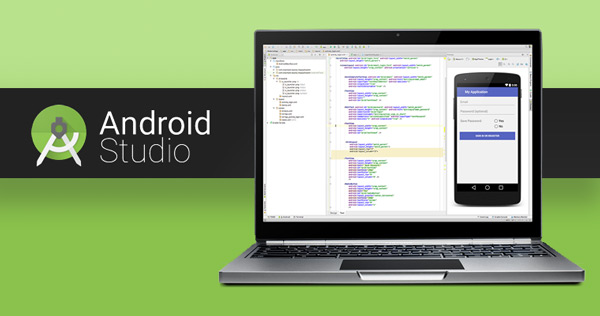
\includegraphics[width=0.6\linewidth]{androidstudio}
	\caption{Android Studio, un IDE flexible e intuitivo.}
	\label{fig:androidstudio}
\end{figure}

Se ha utilizado este IDE frente a otros como Eclipse + ADT \cite{URL::eclipseADT} debido a que en la actualidad es el IDE oficial con soporte de Google. Se ha preferido aprender a utilizar este entorno con vistas al futuro, ya que parece que se consolidará como el preferido para los desarrolladores Android.

Los \textit{``Beacons''} \cite{URL::Beacon} (la traducción del término sería a \textit{``balizas''} o \textit{``faros''}) son una tecnología emergente que desde hace algunos años intenta abrirse paso en el mercado. Como su propio nombre indica, estos dispositivos intentan ser un mecanismo de guía, dando una solución al posicionamiento en interiores, donde otras tecnologías, como el GPS \cite{URL::GPS} o el Wifi dejan de funcionar o resultan imprecisas. Sin embargo, estos no son los únicos usos de los beacons, actualmente muchas empresas están ampliando sus usos a otros campos.


%
% ---------------------------------------------------
%
% Proyecto de Final de Carrera:
% Author: Laura Padrón Jorge <alu0100703511@ull.edu.es>
% Capítulo: Objetivos 
% Fichero: Cap1_Goals.tex
%
% ----------------------------------------------------
%


\chapter{Beacons en entornos universitarios} \label{chap:BeaconsEntornosUniversitarios}  


En este capítulo realizaremos un análisis de los posibles casos de uso de la tecnología beacon en el ámbito universitario.

 
\section{Aplicaciones móviles en entornos universitarios}


En un principio, estas aplicaciones se enfocaban a atraer estudiantes, centrándose en la calidad de la universidad y mostrando las posibilidades que ofrecían. Sin embargo, con el paso de los años y el desarrollo creciente de las aplicaciones móviles, se muestra un cambio en esta estrategia. Ahora las aplicaciones tienen una doble función y no sólo buscan el acceso de nuevos estudiantes, sino que también intentan mejorar la experiencia del alumnado ya matriculado y acercar a los nuevos a la experiencia de la universidad. 
Algunos ejemplos posibles los encontramos en el marketplace de Google \cite{URL::galileo, URL::valladolid, URL::oviedo}


% bliotecaSalamanca.JPG---------------------------------------------------
%
% Trabajo de Fin de Grado. 
% Author: Laura Padrón Jorge. 
% Capítulo: La aplicacion BulletPoint. 
% Fichero: Cap4_TheApplication.tex
%
% ----------------------------------------------------
%

\chapter{La aplicación BulletPoint} \label{chap:LaAplicacion} 

Basándonos en los casos de uso revisados en el capítulo anterior, en este capítulo se discutirán los casos de uso que han sido elegidos e implementados en la aplicación \BulletPoint{}. Comentaremos la aplicación centrándonos en el desarrollo de la misma, así como  en diferentes partes a destacar del código que puedan resultar interesantes.


\section{Casos de uso elegidos}

Como ya hemos mencionado previamente, estos casos de uso se incluyen como parte de la aplicación que se ha desarrollado en este TFG, donde cada caso de uso se considera un módulo. La integración de cada uno de estos módulos con el resto de la aplicación se ha realizado mediante el desarrollo de un menú de funcionalidades donde es posible seleccionar qué acción se desea. Para almacenar la información necesaria para algunos módulos, se ha introducido un menú adicional de ajustes. Estos datos se utilizan entre otras cosas para identificar al usuario y confirmar ciertas acciones o dejar constancia de otras. 


\subsubsection{Funcionamiento}


Mediante el uso de los beacons, permitimos a la aplicación identificar en que parada se encuentra el usuario. La aplicación asocia la MAC \ref{el:mac} de un beacon con el número identificativo de la parada. Este número identificativo de la parada es lo que utiliza TITSA para identificar sus paradas en la API y en toda su web. 


La aplicación ha sido programada enlazando los números identificativos de la parada con la dirección MAC de los beacons. En el listado \ref{code:beaconbusstop} se puede apreciar como se relaciona cada MAC con el número identificativo de la parada.


\lstinputlisting[float, floatplacement=H,caption={\textit{BusBeaconStop}. Esta clase contiene la información que asocia cada MAC con el ID de la parada de TITSA. Añadir un nuevo beacon a una parada implica añadir un nuevo elemento a \textit{stopsMapId}.}, label={code:beaconbusstop}]
{listings/BeaconBusStop.java} %% LISTING


Aparte de esta información, por cada autobús se incluye un enlace a modo de botón que remite al usuario a la página web de TITSA con el identificador de la línea. Así el usuario puede obtener más información adicional en caso de precisarla.

\lstinputlisting[float, floatplacement=H, caption={La clase \textit{Arrival} donde quedan contenidos los datos de cada llegada.}, label={code:arrival}]
{listings/Arrival.java} %% LISTING

\vspace{5mm}
\lstinputlisting[float, floatplacement=H,caption={El handler se encarga de transformar el fichero XML en elementos de tipo \textit{Arrival} (véase Listado \ref{code:arrival}).}, label={code:handler}]
{listings/XmlHandler.java} %% LISTING






%% ---------------------------------------------------
%
% Trabajo de Fin de Grado. 
% Author: Laura Padrón Jorge. 
% Capítulo: Conclusiones y lineas de trabajo futuras. 
% Fichero: Cap5_ConclusionsAndFutureLinesOfWork.tex
%
% ----------------------------------------------------
%

\chapter{Conclusiones y líneas de trabajo futuras} \label{chap:Conclusiones} 

En este capítulo se presentarán las conclusiones a las que se ha llegado tras realizar este TFG y discutiremos posibles líneas de trabajo futuras.

\subsection{Conclusiones}

Actualmente la tecnología beacon se encuentra aún en fase de desarrollo. Por sí sola puede llegar a tener muchas limitaciones debido a su funcionamiento. Las restricciones físicas y de posicionamiento requieren que se realice un análisis para posicionar los dispositivos de la mejor manera. Por otro lado cada distribuidor específico de beacons intenta que se utilicen sus SDKs para desarrollar las aplicaciones. Dependiendo del caso, incluso existen algunos sujetos a cuotas, con lo que desarrollar utilizando esta tecnología puede no resultar económico y poner las cosas difíciles a muchos desarrolladores. La solución a este problema la hemos encontrado en la librería AltBeacon que intenta abrir las puertas a los desarrolladores que pretenden utilizar esta tecnología.


Gracias a esta librería se están desarrollando diferentes aplicaciones, que podrían llegar a tener funcionalidades interesantes para el día a día como la automatización de algunas tareas. Hasta ahora se han explorado las posibilidades más beneficiosas a la hora de vender la tecnología como es la publicidad, pero al desarrollar este trabajo, hemos comprobado que el mercado es mucho más amplio, abarca mucho más de lo que se ha desarrollado hasta ahora. 


La consecución de este TFG muestra que existen muchas aplicaciones que podrían interactuar con esta tecnología y dar lugar a un producto útil y cómodo para los usuarios. En unos años probablemente seamos capaces de explotar al máximo las posibilidades que nos ofrecen los beacons, dando paso a aplicaciones que formen parte de nuestra rutina, sin embargo por ahora seguiremos experimentando con esta tecnología y viendo como evoluciona.


\subsection{Conclusions}

Nowadays, beacon technology is still on a development phase. By itself can be quite limitated due to to its functioning.The physical and positional limitations require a deep analysis in order to place devices the best way. On the other hand, each specific beacon provider tries to use his own SDKs to develop the aplications. Depending on the case, fees might be applied so, working with this technology can end up being not money-saving and make things difficult for many developers.


The solution to this problem has been found on the AltBeacon library, which tries to bring close to developers this technology. Thanks to this library, many applications, which might have handy functionalities for day-to-day usage, have been developed and many related to the automation of tasks. Until now just the advertising possibilites have been explored, since it is the most profitable option. 


However, during this project we have realized that market is far more wide and it covers much more than what has been developed right now. The achievement of this Final Year Project is to show that, many apps able to work with this technology exist and they can give as a result an useful and convenient product for users. 


In a few years, we will probably be able to take advantage of all posibilities beacons offer and we will be able to develop apps, which would end up beeing part of our routine; for now, we will keep on testing this technology and watching it grow.

\subsection{Líneas de trabajo futuras}


En un futuro se podrían ampliar las funcionalidades desarrollando los demás casos de uso planteados que no se han elegido en este trabajo. En entornos universitarios existen multitud de servicios que podemos relacionar con esta tecnología, entre otros podemos destacar: 


\begin{itemize}
\item Acceso a instalaciones deportivas, educativas o de diversa índole.
\item Contratación de servicios en diferentes puntos: alquiler de bicicletas en puntos de alquiler, pago de entradas en las inmediaciones de un evento.
\item Anuncios o promociones de diverso tipo, relacionados tanto con la universidad como con establecimientos comerciales cercanos al campus.
\item Servicios de guía dentro del campus, con puntos de interés para el alumnado.
\end{itemize}


Son múltiples las posibilidades que se le pueden dar a esta tecnología. En otros sectores como el turismo o la medicina también están empezando a tener relevancia, con lo que podemos confirmar que no es una tecnología aislada, sino que poco a poco se está abriendo paso en el mercado.










%% ---------------------------------------------------
%
% Trabajo de Fin de Grado. 
% Author: Laura Padrón Jorge. 
% Capítulo: Presupuesto. 
% Fichero: Cap6_BudgetEstimations.tex
%
% ----------------------------------------------------
%

\chapter{Presupuesto y puesta en marcha} \label{chap:presupuesto} 

En este capítulo se expondrán las estimaciones de recursos necesarios para poner en práctica este despliegue teniendo en cuenta el estado actual del proyecto. 

El desglose del presupuesto de la aplicación se puede separar en dos partes: por un lado, la compra de los distintos dispositivos, y por otro el desarrollo y mantenimiento de la aplicación. Se puede contabilizar de la siguiente manera: 

\begin{itemize}
\item Para el caso de uso de los autobuses, sería necesario un beacon por parada. Si sólo se cubriesen las paradas dentro de la zona universitaria, obtendríamos unos 20 beacons a distribuir entre Anchieta y Guajara.
\item Siguiendo con el caso de uso de los eventos, se podrían calcular  10 zonas de eventos principales nuevamente a distribuir entre Guajara y Anchieta. Estas zonas abarcarían desde el paraninfo, aulas magnas o bibliotecas hasta lugares destinados específicamente para la realización de eventos.
\item Para los casos de uso que dependen de la localización, debemos realizar un análisis de cada recinto: los aparcamientos para el módulo del aparcamiento, las aulas para el módulo de asistencia y los edificios o exteriores para el módulo de guía.
\end{itemize}

Teniendo en cuenta que cada dispositivo de Aruba lo comercializamos por 25 euros:

 
\begin{itemize}
\item Para cubrir el primer caso de uso sería necesaria una inversión de 500 euros y cubriríamos 20 paradas de autobús.
\item Para las 10 zonas de eventos se necesitarían 250 euros (aunque es posible añadir más beacons)
\item Los casos de uso que dependen de la localización son relativos: como hay 8 aparcamientos y se necesitan como mínimo 3 beacons por recinto, podríamos hablar de un mínimo de 600 euros a desembolsar. En el caso de la asistencia y guía, si calculamos  que para cubrir todos los edificios de la ULL (facultades en su mayoría) se necesitarían unos 100 beacons, el importe asciende a 2500 euros.
\end{itemize}


Esta primera parte del presupuesto suma en total 3.850 euros y con ellos quedarían cubiertos los edificios, aparcamientos y paradas de autobús cercanas al campus. La instalación y configuración de los dispositivos se ha calculado en base a la suma de 12,40 euros por hora trabajada. Se necesitarían 2 especialistas trabajando durante un mes a jornada completo (8 horas) para realizar la instalación.

El total del despliegue ascendería a 3.968 euros. Si lo sumamos al precio de los dispositivos obtenemos la suma de 7.818 euros. Los dispositivos cuentan con una garantía de un año por lo que, si el dispositivo fuese considerado defectuoso en ese plazo, se procedería al cambio del mismo sin coste para el cliente.


Aparte de los dispositivos hay que añadir la segunda parte del coste, derivada del mantenimiento de la aplicación y  del coste de un servidor para almacenar los datos y realizar las consultas. Para esta parte se ofrecen dos opciones: 

\begin{itemize}
\item Compra del servidor dedicado junto con el soporte y configuración servidor (cuota anual) : 1300 + 250 = 1.550 euros.
\item Configuración de un servidor ya disponible en la Universidad (sin cuota anual de soporte ni mantenimiento): 550 euros. 
\end{itemize}


Por otro lado, sería recomendable el mantenimiento de la aplicación. Ofrecemos un especialista programador en Android que se haría cargo de las incidencias que pudieran surgir con la app en horario laboral a jornada completa, con un tiempo de respuesta de 24 horas y solución de la incidencia en 72 horas a partir de la confirmación de la misma.

El coste final ascendería a 21.600 euros anuales netos durante el primer año y a 18.000 euros en adelante. Este mantenimiento no incluye nuevas funcionalidades, únicamente el mantenimiento y el correcto funcionamiento de los módulos disponibles a día de hoy.

 
El presupuesto final habría que calcularlo en función de las distintas opciones presentadas.


%\newpage{\pagestyle{empty}}
%\thispagestyle{empty}

%\chapter{Presupuesto}
%\label{chapter:Presupuesto}

%\input{cap7.tex}

%%%%%%%%%%%%%%%%%%%%%%%%%%%%%%%%%%%%%%%%%%%%%%%%%%%%%%%%%%%%%%%%%%%%%%%%%%%%%%%

%%%%%%%%%%%%%%%%%%%%%%%%%%%%%%%%%%%%%%%%%%%%%%%%%%%%%%%%%%%%%%%%%%%%%%%%%%%%%%%
%\newpage{\pagestyle{empty}}
%\thispagestyle{empty}
%\begin{appendix}
%
%\chapter{Título del Apéndice 1}
%\label{appendix:1}
%\input{apendice1.tex}
%
%\chapter{Título del Apéndice 2}
%\label{appendix:2}
%\input{apendice2.tex}
%
%\end{appendix}
%%%%%%%%%%%%%%%%%%%%%%%%%%%%%%%%%%%%%%%%%%%%%%%%%%%%%%%%%%%%%%%%%%%%%%%%%%%%%%%
\addcontentsline{toc}{chapter}{Bibliografía}
%\bibliographystyle{plain}
\bibliographystyle{bmc_article} 
\renewcommand{\bibname}{Bibliografía}   %  Para que no aparezca Índice de figuras
\bibliography{bibliografia}

%%%%%%%%%%%%%%%%%%%%%%%%%%%%%%%%%%%%%%%%%%%%%%%%%%%%%%%%%%%%%%%%%%%%%%%%%%%%%%%

\end{document}
